\documentclass{standalone}
\usepackage{tikz}
\usetikzlibrary{calc, shapes, backgrounds}
\usepackage{standalone}
\usepackage{amsmath, amssymb}
\pagecolor{olive!50!yellow!50!white}
\begin{document}

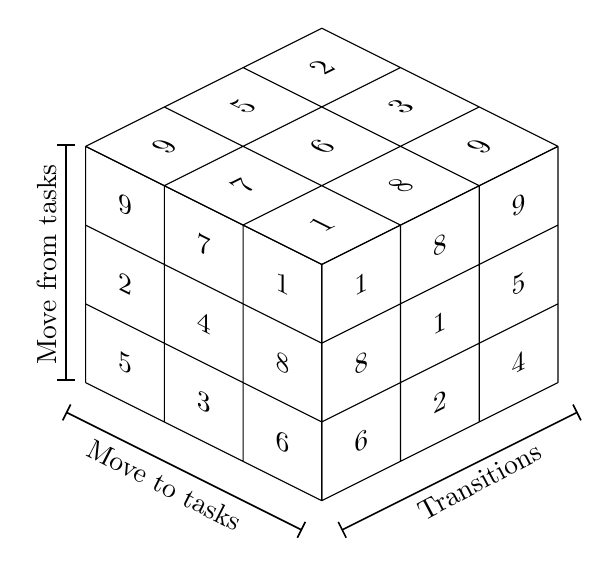
\begin{tikzpicture}
\begin{scope}[every node/.append style={yslant=-0.5},yslant=-0.5]
  \node at (0.5,2.5) {9};
  \node at (1.5,2.5) {7};
  \node at (2.5,2.5) {1};
  \node at (0.5,1.5) {2};
  \node at (1.5,1.5) {4};
  \node at (2.5,1.5) {8};
  \node at (0.5,0.5) {5};
  \node at (1.5,0.5) {3};
  \node at (2.5,0.5) {6};
  \draw (0,0) grid (3,3);
\end{scope}
\begin{scope}[every node/.append style={yslant=0.5},yslant=0.5]
  \node at (3.5,-0.5) {1};
  \node at (4.5,-0.5) {8};
  \node at (5.5,-0.5) {9};
  \node at (3.5,-1.5) {8};
  \node at (4.5,-1.5) {1};
  \node at (5.5,-1.5) {5};
  \node at (3.5,-2.5) {6};
  \node at (4.5,-2.5) {2};
  \node at (5.5,-2.5) {4};
  \draw (3,-3) grid (6,0);
\end{scope}
\begin{scope}[every node/.append style={
    yslant=0.5,xslant=-1},yslant=0.5,xslant=-1
  ]
  \node at (3.5,2.5) {9};
  \node at (3.5,1.5) {7};
  \node at (3.5,0.5) {1};
  \node at (4.5,2.5) {5};
  \node at (4.5,1.5) {6};
  \node at (4.5,0.5) {8};
  \node at (5.5,2.5) {2};
  \node at (5.5,1.5) {3};
  \node at (5.5,0.5) {9};
  \draw (3,0) grid (6,3);
\end{scope}

%x-axis
\draw[|-|,semithick,yslant=-0.5] (-0.25,-0.5) -- (2.75,-0.5);
\draw (1,-1.3) node[rotate= -27] {Move to tasks};

%y-axis
\draw[|-|,semithick,yslant=-0.5] (-0.25,-0.1) -- (-0.25,2.9);
\draw (-0.25,1.5) node[rotate=90, anchor= south] {Move from tasks};

%z-axis
\draw[|-|,semithick,yslant=-0.5] (3.25,-0.25) -- (6.25,2.75);
\draw (5,-1.25) node[rotate=28] {Transitions};
\end{tikzpicture}
\end{document} 
